\documentclass{ctexart}

%	graphicx宏包
%	\includegraphics[keyvals]{imagefile}
%	格式:eps pdf png jpeg bmp
%	help: texdoc graphicx
%	灵活使用图片表格需要使用浮动体
%	h(here)该位置
%	t(top) 同下
%	b(bottom)此页底部,下页底部
%	p(page)独立一页 

%	标题可以使用caption bicaption
%	并列与子图表subcaption subfig floatrow
%	绕排picinpar wrapfig
\usepackage{graphicx}
%\graphicspath{{figures/}}

\begin{document}
	
	\section{图片}
	\LaTeXe{}1中的插图,请见图\ref{figure_01}:
	\begin{figure}[htbp]	%	浮动体
		\centering
		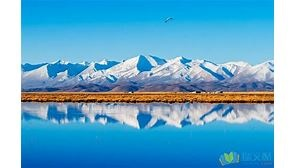
\includegraphics[scale = 2]{view}
		\caption{风景图1}	%	设置标题
		\label{figure_01}	%	设置标签,交叉引用
	\end{figure}

	\LaTeXe{}2中的插图,请见图\ref{figure_02}:
	\begin{figure}[htbp]	%	浮动体
		\centering
		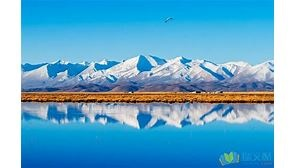
\includegraphics[scale = 2]{view}
		\caption{风景图2}	%	设置标题
		\label{figure_02}	%	设置标签,交叉引用
	\end{figure}

	\LaTeXe{}3中的插图,请见图\ref{figure_03}:
	\begin{figure}[htbp]	%	浮动体
		\centering
		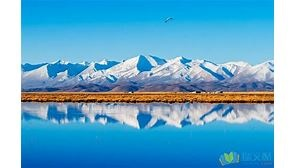
\includegraphics[scale = 2]{view}
		\caption{风景图3}	%	设置标题
		\label{figure_03}	%	设置标签,交叉引用
	\end{figure}
	
	
	\section{表格}	%	texdoc	booktab longtab tebu
	大学生的成绩,请见表\ref{table_01}:
	
	\begin{table}[htbp]	%	浮动体
		\centering
		\begin{tabular}{l || c | p{1.5cm}}% 对齐方式,|分割,p{}指定宽度
			\hline	%	表格横线
			姓名 & 年龄 & 分数\\
			\hline	\hline	%	表格横线
			wang & 18 & 90\\
			li & 19 & 70\\
			zhao & 18 & 80\\
			\hline	%	表格横线
		\end{tabular}
		\caption{分数表}	%	设置标题
		\label{table_01}	%	设置标签
	\end{table}
	
	
	
\end{document}